% !TEX root = omar-thesis-proposal.tex
\vspace{-25pt}
\section{Motivation}\label{motivation}
Specifying and implementing a programming language together with its supporting tools (collectively, a \emph{programming system}) that is built upon sound theoretical foundations, helps users identify and fix errors as early as possible, supports a natural programming style, and performs well across diverse problem domains and hardware platforms remains a grand challenge in computing. In view of this goal, researchers and domain experts (collectively, \emph{providers}) continue to develop new special-purpose syntax, static and dynamic semantics, implementation strategies, optimizations, run-time systems and tools (collectively, \emph{features})  designed to address these challenges in increasingly diverse contexts. Ideally, a provider would be able to develop and distribute these kinds of new features orthogonally, as libraries, so that client developers could granularly choose those that best satisfy their needs. Unfortunately this is often infeasible because from the perspective of a library, the language's syntax and semantics are fully specified in advance, the compiler and run-time system are ``black box'' implementations of this fixed specification, and the other tools, like code editors and debuggers, operate according to fixed protocols. Providers of new system features must, as a result, take \emph{language-external approaches}, often by deriving a new programming system altogether. This approach has been encouraged, historically, by the availability of tools like compiler generators and language workbenches. We will argue that these approaches are technically problematic and that taking them has led to an unnecessary gap between research and practice. In their place, we will develop \emph{language-integrated extensibility mechanisms} that decentralize control over several core aspects of the programming system. By organizing new features around {types} and constraining them appropriately, we aim to show that these mechanisms can guarantee safety and non-interference of extensions while remaining highly expressive.
%But taking a \emph{language-internal approach} to implementing a feature is the most practical. If a feature can be realized by creatively using existing language constructs and distributed as a library, clients face fewer barriers to adoption because it is easy to integrate library-based features into existing projects gradually and granularly and they leverage well-understood and well-developed mechanisms.
% But taking this approach is often \emph{not} possible today %We call designs \emph{monolithic programming systems}.

%To realize a new abstraction or system behavior, such experts can consider either a \emph{language-internal approach}, where they work within an existing language and distribute their solutions as libraries, or a \emph{language-external approach}, where they create a new, distinct programming system (often centered around what has come to be called a new \emph{domain-specific language} \cite{dsl}) or extend an existing system by some mechanism that is not part of the language itself, such as an extension mechanism supported by a {particular} compiler, editor or other tool.
\subsection{Motivating Example: Regular Expressions}\label{regex}
To make the problem we aim to address concrete, we begin with a simple example that we will return to throughout this work. \emph{Regular expressions} are a widely-used abstraction for finding patterns in semi-structured strings (e.g. DNA sequences) \cite{Thompson:1968:PTR:363347.363387}. If a programming system wished to fully support regular expressions, it might simultaneously provide features like these:

\begin{enumerate}
\item \textbf{Syntax for pattern literals} so that the cognitive load of reading and writing patterns is low, patterns are parsed once at compile-time and malformed patterns result in intelligible {compile-time} errors.
\item A \textbf{static semantics} that ensures that key invariants related to regular expressions are maintained:
	\begin{enumerate}
	\item only other patterns and properly escaped strings are interpolated into a pattern, to avoid splicing errors and injection attacks \cite{owasp2013, Bravenboer:2007:PIA:1289971.1289975}
	\item out-of-bounds backreferences are not used \cite{spishak2012type}
	\item string processing operations do not lead to a string that is malformed, when well-formedness can be captured by a regular expression \cite{fulton-thesis}
	\end{enumerate}
When an error is found, an intelligible error message is provided.
%\item An \textbf{implementation} that partially or fully compiles known regular expressions into the efficient internal representation that will be used by the regular expression matching engine (e.g., a finite automata \cite{Thompson:1968:PTR:363347.363387}) ahead of time. In most languages, this compilation step occurs at run-time, even if the pattern is fully known at compile-time, thereby introducing performance overhead into programs. If the developer is not careful to cache compiled representations, regular expressions used repeatedly in a program might be needlessly re-compiled on each use. %By performing this step ahead-of-time, these dangers can be avoided.
\item \textbf{Editor services} that allow clients to interactively test regular expression patterns against test strings, refer to documentation or search for common patterns (e.g. \cite{IntelliJRegexp}).
\end{enumerate}

%In a conventional \emph{monolithic} programming system, support for each of these features would need to be built into the language and tools. 
No system today builds in support for all of the features enumerated above in their strongest form. Instead, libraries generally provide support for regular expressions by leveraging  general-purpose abstraction mechanisms. Unfortunately, it is impossible to fully define the syntax and the specialized static semantics described in the references above in terms of general-purpose notations and abstractions. Library providers thus need to compromise. The most common strategy is to ask clients to enter patterns as strings deferring their parsing, typechecking, compilation and use to run-time. This proves only a weak approximation to feature 1 (due to clashes between string escape sequences and regular expression syntax). None of the static guarantees can be provided in this way, leading to run-time exceptions (even in well-tested code, as shown in \cite{spishak2012type}), and logic errors that are not caught even at run-time, some of which can lead to security vulnerabilities (due to injection attacks, for example \cite{owasp2013}). It also introduces performance overhead (due to run-time parsing and compilation of patterns, and potentially redundant run-time string checks). Requiring that clients instead introduce patterns directly using general-purpose constructs like object or inductive datatype constructors or operations over an abstract type rather than via strings can only provide feature 2a while eliminating even the weak approximation to feature 1 that the use of string literals provides. 

None of these approaches address the issue of tool support. Regular expressions are not trivial to work with, so tool support can be quite helpful, even for experts, and a number of tools are available online. Unfortunately, tools that must be discovered independently and accessed externally are used infrequently \cite{Murphy-Hill:2011:PIE:1958824.1958888} and are less usable than editor-integrated tools \cite{Campbell:2008:DRT:1636642.1636651, Omar:2012:ACC:2337223.2337324}, leading to lower productivity.

\subsection{Language-External Approaches}\label{external-approaches}
\begin{figure}
\begin{center}
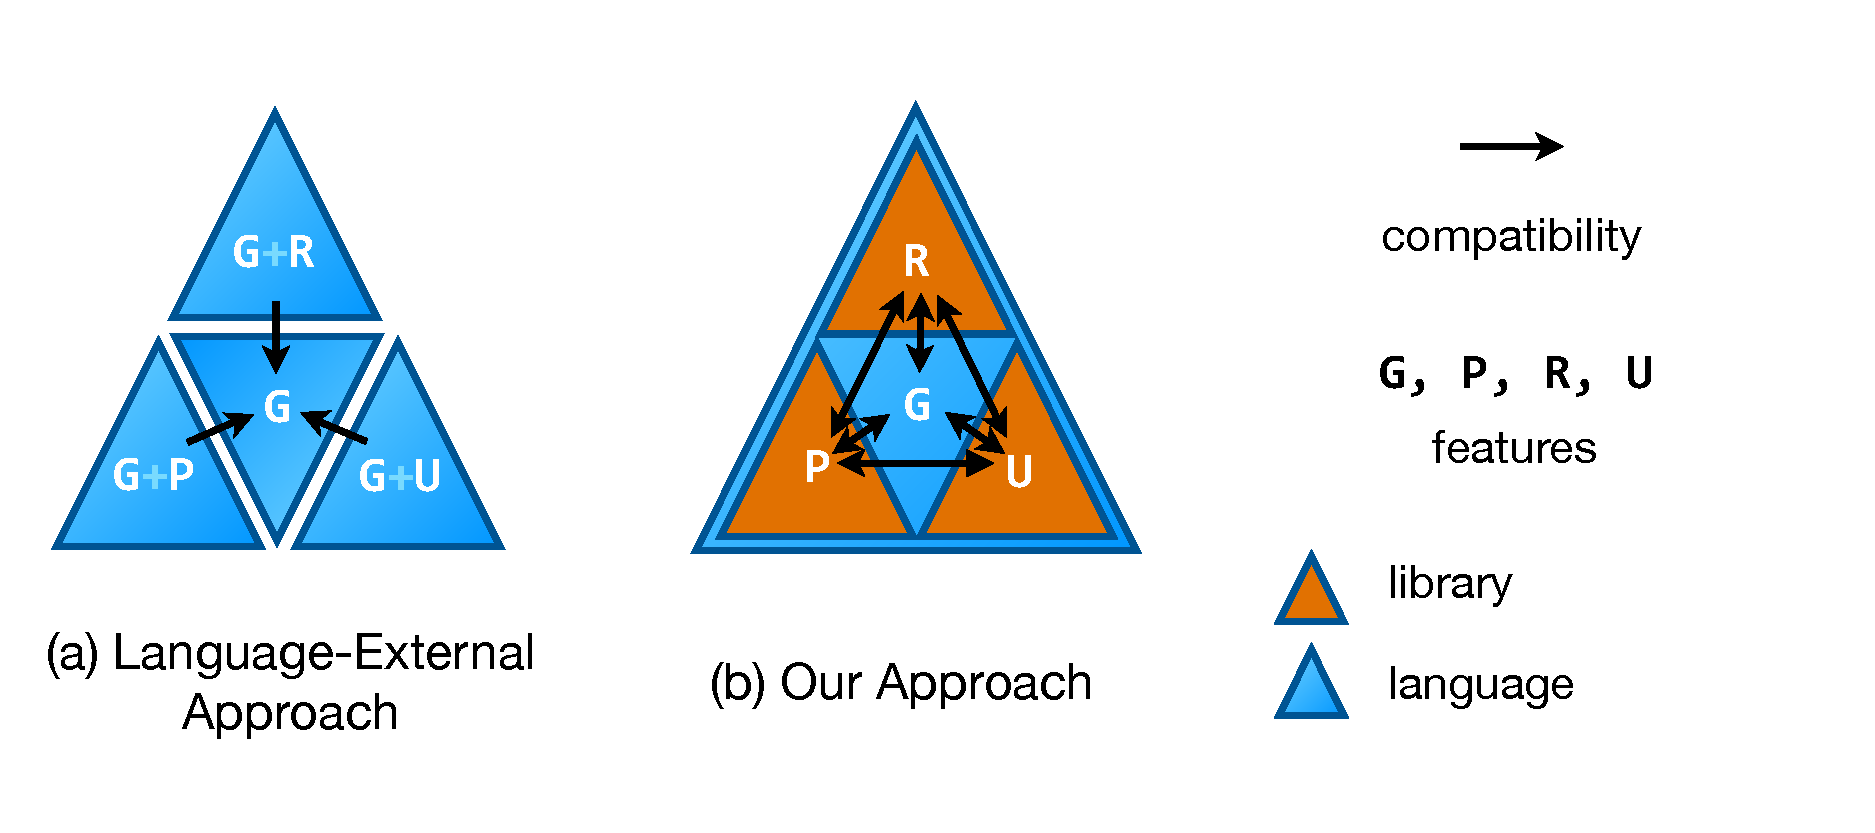
\includegraphics[scale=.48]{approaches.pdf}
\end{center}
\vspace{-20px}
\caption{\small (a) When taking a language-external approach, new features are packaged together into separate languages and tools, causing problems with orthogonality and client compatibility (described in the text). (b) When taking a language-integrated approach, there is one extensible host language and the compile-time and edit-time logic governing new constructs is expressed within ``active'' libraries. If the extension mechanism guarantees that extensions cannot interfere with one another or the base system, these problems are avoided.}
\label{approaches}
%\vspace{-10px}
\end{figure}

When the syntax and semantics of a system must be extended to fully realize a new feature, as in the example above and others we will give throughout this work, providers typically take a \emph{language-external approach}, either by developing a new or derivative programming system (supported by \emph{language workbenches} \cite{erdweg2013state},  \emph{DSL frameworks} \cite{fowler2010domain} or \emph{compiler generators} \cite{brooker1963compiler}), or by extending an existing artifact, such as an extension mechanism for a {particular} compiler\footnote{Compilers that modify, or allow modification of, the semantics of their base language, rather than simply permitting semantics-preserving optimizations, should be considered a pernicious means for creating new languages. Many ``practical'' compilers, including \texttt{gcc}, \texttt{GHC} and \texttt{SML/NJ}, are guilty of this, meaning that some programs that seem to be written in C, Haskell or Standard ML are actually written in tool-specific derivatives of these languages. Language-integrated mechanisms do not lead to such fragmentation.}, editor or other tool. For example, a researcher interested in providing regular expression related features (let us refer to these collectively as \texttt{R}) might design a new system with built-in support for these, perhaps basing it on an existing system containing some general-purpose features (\texttt{G}). A different researcher developing a new language-integrated parallel programming abstraction (\texttt{P}) might  take the same approach. A third researcher, developing an alternative parallel programming abstraction (\texttt{Q}) might again do the same. This results in a collection of distinct systems as diagrammed in Figure \ref{approaches}a. Unfortunately, when providers of new features take language-external approaches like this, it causes  problems for clients related to \textbf{orthogonality} and \textbf{client compatibility}. %This latter method couples the semantics of the feature to the implementation details of a particular tool. Because the use of one implementation entails a different semantics for the feature than another, the extended tool acts, \emph{de facto}, as a distinct system for our purposes. 

\paragraph{Orthogonality} Features implemented by language-external means cannot be adopted individually, but instead are only available coupled to a fixed collection of other features. This makes adoption more costly when these incidental features are  not desirable or insufficiently developed, or when the features bundled with a different language or tool are simultaneously desirable. That is, one must either use the system containing features \texttt{G+R}, \texttt{G+P} or \texttt{G+Q}. There is no system containing \texttt{G}, \texttt{R}, \texttt{P} and \texttt{Q} in other combinations, and merging the systems containing each separately can be non-trivial because there is no requirement that providers of new features use a common mechanism. Even in cases where a common mechanism has been used, there are serious interference and safety issues, as we will discuss at length throughout this thesis.

Recent evidence indicates that this is one of the major barriers preventing research from being driven into practice: developers prefer language-integrated parallel programming abstractions with stronger safety guarantees and more natural syntax to library-based abstractions if all else is equal \cite{cave2010comparing}, but library-based implementations are more widely adopted because ``parallel programming languages'' privilege only a few chosen  abstractions at the language level. This is problematic because different parallel programming abstractions are seen as more appropriate in different situations \cite{Tasharofi:2013rc}. Moreover,  parallel programming support is rarely the only concern relevant to client developers outside of a classroom setting. Regular expression support, for example, may be simultaneously desirable for processing large amounts of textual data in parallel, but using these features together in the same compilation unit would be difficult or impossible.  %Similarly, a language and tools designed primarily to support regular expressions might make an interesting research project, but it would not be a suitable tool for writing large applications with more varied needs.

%\item Developing a new language and its associated tools places a significant development burden on providers who may wish only to promote a few core innovations, although tools like compiler generators, language workbenches and easy-to-extend tools can decrease this burden. 
%\item 

%Clients seem to prioritize the ability to choose different features for different portions of an application. 
%If calling between languages were safe and easy, then using a variety of specialized languages and associated tools might be less problematic. In fact, s
%Recognizing the limitations of relying on monolithic collection of primitives, some researchers have advocated instead for a model where multiple languages used within a single application, calling it the \emph{language-oriented approach} to software development \cite{languageoriented}. 

\paragraph{Client Compatibility} Even in cases where for each component of a software system there is a programming system that is completely satisfactory in isolation, there remain problems at the interface between components. An interface that exposes the specialized constructs particular to one language (e.g. futures in a parallel programming language) cannot necessarily be safely and naturally consumed from another language (e.g. a general-purpose language). Tool support is also lost when calling into a different language. We call this fundamental issue the \emph{client compatibility problem}: code written by clients of a certain collection of features cannot always interface with code written by clients of a different collection  in a safe, performant and natural manner.

One strategy often taken by proponents of a \emph{language-oriented approach} to software development \cite{journals/stp/Ward94} to partially address the client compatibility problem is to  target an established intermediate language, such as the Java Virtual Machine (JVM) bytecode, and use its constructs as a common language for communication between components written in different languages. Scala \cite{200464/IC} and F\# \cite{pickering2007foundations} are examples of prominent general-purpose languages that have taken this approach, and most DSL frameworks also rely on this strategy. As indicated in Figure \ref{approaches}a, this only enables client compatibility in one direction. Calling into the common language becomes straightforward and safe, but calling in the other direction, or between the languages sharing the common target, does not. 

This approach can work well when new languages consist of constructs that can also be expressed safely and almost as naturally in the common language.
But many of the most innovative constructs found in modern languages (often, those that justify their creation) are difficult to define in terms of existing constructs in ways that guarantee all necessary invariants are statically maintained and that do not require large amounts boilerplate code and run-time overhead. As a trivial example with significant practical implications, F\#'s type system does not admit \verb|null| as a value for any type defined within F\# code, but maintaining this important invariant still requires run-time checks because the typing rules of F\# do not apply when F\# data structures are constructed by other languages on the Common Language Infrastructure (CLI) like C\# or SML.NET. This is not an issue exclusive to intermediate languages that make regrettable choices regarding \verb|null|, however. The F\# type system also includes support for checking that units of measure are used correctly \cite{syme2012expert, kennedy1994dimension}, but this more specialized invariant is left unchecked at language boundaries. No alternative  general-purpose intermediate language would change this situation. %Even exposing datatypes  and tuples at component boundaries, which are used ubiquitously and can be safely consumed from other languages, is not recommended when a component might be used from another language, according to drafted F\# component design guidelines \cite{fsharpguidelines}, because these are awkward to consume from other languages without the convenient primitive operations (e.g. pattern matching) and syntax that F\# includes. SML.NET prohibits exposing such types at component boundaries altogether. 
%In Scala, traits that have default method implementations are difficult to implement from Java or other JVM languages and the workaround can break if the trait is modified \cite{scalatraitinterop}. 
%In some cases, desirable features must be omitted entirely due to concerns about interoperability. F\#, for example, aimed to retain source compatibility with Ocaml code, but due to the need for bidirectional interoperability with CLI languages, it does not support features like polymorphic variants, modules or functors \cite{ocaml-manual} because they have no apparent analogs in the type system of the CLI.
%\end{itemize}

\subsection{Language-Integrated Approaches}\label{language-integrated-approaches}
We argue that, due to these problems with orthogonality and client compatibility, taking a language-external approach to realizing a new feature should be considered harmful and avoided whenever possible. The goal of the research being proposed here is to design \emph{language-integrated extension mechanisms} that give providers the ability to define, within libraries, new features that have previously required central planning, 
%\footnote{One might compare today's programming systems to  {centrally-planned} economies, whereas extensible\- systems more closely resemble modern market economies. Our safety constraints serve a role analagous to market regulation. We leave further development of this analogy to the reader.}
so that language-external approaches are less frequently necessary. More specifically, we will show how control over aspects of the \textbf{syntax}, \textbf{static and dynamic semantics} and \textbf{editor services} can be delegated to user-defined logic distributed in {libraries}, as illustrated in Figure \ref{approaches}b. 
Such libraries have been called \emph{active libraries}  \cite{activelibraries} because, rather than being passive clients of features already available in the system, they contain logic invoked by the system during development or compilation to provide new features. Features implemented within active libraries can be imported as needed, unlike features implemented by external means, seemingly avoiding the problems of orthogonality and client compatibility.

We must proceed with caution, however: critical issues having to do with {safety} must be overcome before language-integrated extension mechanisms can be integrated into a system. If too much control over  these core aspects of the system is given  to developers, the system may become quite unreliable. 
%For example, an extension could weaken important metatheoretic guarantees previously provided by the system. 
Type safety, for example, may not hold if the static and dynamic semantics of the language can be modified or extended arbitrarily from within libraries. Furthermore, even if extensions can be shown not to cause such problems in isolation, there may still be conflicts between extensions that could weaken their semantics, leading to subtle problems that only appear when two extensions are used together. For example, if two active libraries introduce the same syntactic form but back it with differing (but individually valid) semantics, the issue would only manifest itself when both libraries were imported somewhere within the same scope. These kinds of safety issues have plagued previous attempts to design language-integrated extensibility mechanisms. We will briefly review some of these attempts below.% To prevent them, our mechanisms will organize  extension logic around types to guarantee that extensions are both safe in isolation and also safely composable in any combination. 


 %This represents a minimalist approach to system design -- the conventional distinction between built-in and user-defined constructs is blurred and most features of the system are orthogonally implemented as {libraries}, rather than by the maintainers of the system.

%The mechanisms we describe will do so primarily by delimiting the scope of an extension to expressions of a single user-defined type or family of types. 

%This can be thought of as a more pernicious form of the conflict that arises when two globally-accessible constructs are given the same name. n languages without universal namespacing mechanisms (e.g. C, JavaScript, \LaTeX, ML and many others). 

%The extension mechanism\todo{elaborate on safety requirements + tension between expressiveness and safety, merge with next paragraph}. must be expressive enough to allow users to associate rich run-time, compile-time and edit-time behaviors with user constructs directly, while being sufficiently restrictive to maintain the global safety properties of the language and system as a whole, and to ensure that constructs cannot interfere with one another. 
